\documentclass[class=NCU_thesis, crop=false]{standalone}
\begin{document}

\chapter{相關研究}
本章節中,
將說明有關本研究之背景知識與文獻回顧,
透過以下四章子節進行分述:
嬰兒猝死症、嬰兒監測系統、殘差神經網路及人臉偵測演算法。

\section{嬰兒猝死症}
嬰兒猝死症(The Sudden Infant Death Syndrome, 簡稱SIDS)~\cite{kinney_sudden_2009}
其特徵為一位看似健康的嬰兒在睡眠期間突然死亡,
其真正致死之原因尚不明確且非單一。

目前醫界對嬰兒猝死症之直接致死原因尚未有統一的定義,
但可統整出多項促使此症發生之風險因素,
主要可分為兩類:
其一為外在因素,包含嬰兒因俯臥及側睡姿勢、蓋住臉部的床單、嬰兒睡在沙發或其他容易陷入的柔軟家具上等,
致使嬰兒呼吸困難而死亡;
其二則為內在因素,
包含成長因素(如:早產)、
遺傳因素(如:家族性之嬰兒猝死症)、
性別(男性比例為女性的兩倍)或種族等。
除此之外,嬰兒也可能因其他外在環境條件,
如:產前或產後暴露於不良物質中(如:香菸煙霧、酒精或非法藥物等),
而弱化嬰兒之內在條件。

在嬰兒猝死症研究中,
有許多關於此症之死亡機制理論,
其中心肺控制假說主導了多數研究,
也造就了往後關於此症之探討多基於嬰兒呼吸或自主神經機制的缺陷。
此論點主要包含了五個步驟:
(1)發生危及生命的事件(如:面部朝下或面部遭遮蔽,造成反射性或阻塞性呼吸暫停),
而將導致嬰兒窒息或腦部灌注不足,亦可能兩者皆發生。
(2)嬰兒無法自行轉頭,以應對窒息的情境,而導致無法從呼吸暫停中恢復。
(3)持續性窒息導致嬰兒失去意識或反射,即低氧昏迷。
(4)發生心率過緩及缺氧喘氣,此現象在嬰兒因嬰兒猝死症逝世前將明顯發生。
(5)嬰兒的自主復甦能力受損,即因無效的喘氣而最終導致呼吸暫停及死亡。
因此,由嬰兒猝死症之紀錄中,
可看出此症並非一種突發疾病,
而是在嬰兒死亡前,
即會出現心率不正常或呼吸暫停之惡性循環現象。

另外,
亦有研究人員使用Triple-Risk Model來解釋嬰兒猝死症~\cite{noauthor_what_nodate},
即嬰兒死於此症需同時包含以下三個因素:
(1)有風險的嬰兒:嬰兒含有一個未知的問題,可能是基因突變或腦部缺陷等,這使其面臨了嬰兒猝死症的風險;
(2)嬰兒發育的重要時期:嬰兒出生後的前六個月,將經歷許多快速成長的階段,此階段會改變身體控制和調節自身的能力,且嬰兒的身體也會於此時學習如何對環境做出應變;
(3)環境中的壓力源:即前述中之外在因素,包含嬰兒睡姿及接觸香菸煙霧等。
若僅發生其中一項因素,
將不足以導致嬰兒猝死症引發死亡。

因此,
若能消除環境中的壓力源,
將有利於嬰兒的生存。
同時醫界亦發現俯臥睡姿勢將使嬰兒猝死症風險增加三倍以上,
故在1990年代初期國際間即提倡嬰兒仰臥睡姿,
此症之發病率也因此降低了50\% 以上,
但仍為嬰兒主要死亡原因之一。

\section{嬰兒監測系統}
由於嬰兒尚無能力表達且無法避免危險,
因此,為了協助照顧者關注嬰兒狀態,
現有許多為自動化監測嬰兒之研究,
主要分為以感測器偵測生理訊號及以影像式偵測兩種方式。
% 兩種方式的優缺點比較

\subsection{感測器偵測}
此種方式利用呼吸感測器、濕度感測器、溫度感測器、慣性感測器、三軸加速度計、一氧化碳感測器及二氧化碳感測器等多種不同設備,
進行嬰兒呼吸頻率、出汗狀況、體溫、心率、身體位置或方向、睡眠姿勢、周圍一氧化碳濃度及呼出的二氧化碳濃度變化等訊號之偵測,
且多會透過物聯網技術開發出可穿戴式裝置,
以下介紹幾項基於感測器式偵測嬰兒之研究。

Linti等人~\cite{linti_sensory_2006}將多個感官元件融入紡織品以開發嬰兒感測背心,
此裝置可用來量測嬰兒之呼吸、心率、溫度及濕度,
其示意圖見\cref{fig:fig-linti_sensory_2006}。
\fig[0.7][fig:fig-linti_sensory_2006][!hbt]{fig-linti_sensory_2006.png}[Linti嬰用感測背心之穿脫示意圖~\cite{linti_sensory_2006}][Linti嬰用感測背心之穿脫示意圖~\cite{linti_sensory_2006}]

Ferreira等人~\cite{ferreira_smart_2016}將心律感測器、3D加速度計、熱電堆感測器裝設於胸帶中(\cref{fig:fig-ferreira_smart_2016}),
以量測嬰兒之體溫、心率、呼吸頻率及身體位置,
再透過ZigBee技術傳送數據至伺服器,
並可由網頁查收訊息。
\fig[0.7][fig:fig-ferreira_smart_2016][!hbt]{fig-ferreira_smart_2016.png}[Ferreira嬰用感測胸帶~\cite{ferreira_smart_2016}][Ferreira嬰用感測胸帶~\cite{ferreira_smart_2016}]

Lin等人~\cite{lin_wireless_2014}於胸帶中嵌入三軸加速度計、溫度感測器及一氧化碳感測器,
可用來量測嬰兒睡姿(面朝上、下、左或右)、體溫及其周圍一氧化碳濃度,
且利用三軸加速度計z軸資訊可獲得嬰兒之呼吸頻率,
最終驗證計算之呼吸頻率準確率達100\%。
此系統架構圖見\cref{fig:fig-lin_wireless_2014},
\fig[0.7][fig:fig-lin_wireless_2014][!hbt]{fig-lin_wireless_2014.png}[Lin系統架構圖~\cite{lin_wireless_2014}][Lin系統架構圖~\cite{lin_wireless_2014}]

Ziganshin等人~\cite{ziganshin_uwb_2010}
基於超寬頻技術開發出可監測呼吸及心率之系統(如\cref{fig:fig-ziganshin_uwb_2010}),
以檢測嬰兒三種狀態:睡眠(無運動)、清醒(長期大幅度運動)及警示(偵測到呼吸頻率異常低或暫停)。
\begin{figure}[!hbt]
    \centering
    \subcaptionbox
        {正常狀態
        \label{fig:fig-ziganshin_uwb_2010-01}}
        {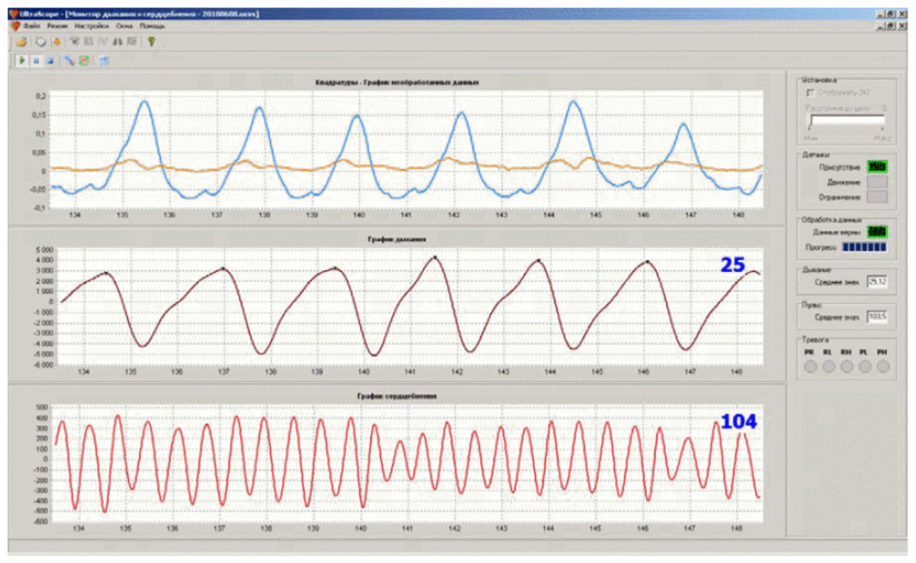
\includegraphics[width=0.45\linewidth]{fig-ziganshin_uwb_2010-01}}
    ~
    \subcaptionbox
        {呼吸暫停狀態
        \label{fig:fig-ziganshin_uwb_2010-02}}
        {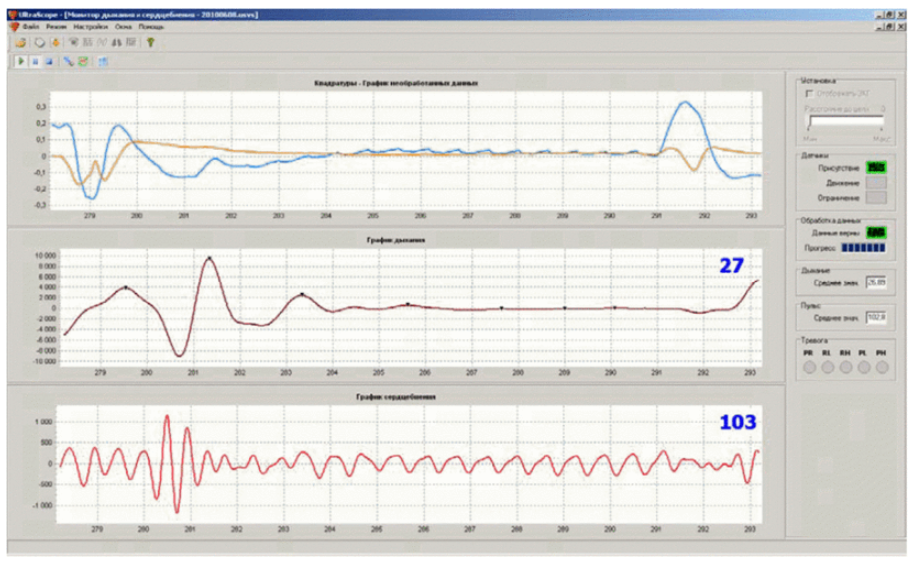
\includegraphics[width=0.45\linewidth]{fig-ziganshin_uwb_2010-02}}
    \caption{Ziganshin系統之嬰兒呼吸及心跳圖~\cite{ziganshin_uwb_2010}}
    \label{fig:fig-ziganshin_uwb_2010}
\end{figure}

此種利用感測器監測嬰兒的方法,
雖然可直接量測其生理訊號以判斷狀態正常與否,
但仍可能因硬體設備之缺陷無法準確量測,
進而有失判斷準確性,
亦或者因需額外穿戴裝置而造成嬰兒不適,
進而影響活動或導致更多危險的發生。

\subsection{影像式偵測}
現有研究中,
基於電腦視覺技術之監測系統雖日漸廣泛,
但多針對小孩、成人或老人之照護進行開發,
而少數應用於嬰兒的偵測系統中,
又多關注於呼吸頻率、面部特徵及趴睡姿勢等,
以下介紹幾項基於影像式偵測嬰兒之研究。

有別於往的接觸式或非視覺技術之呼吸頻率偵測系統,
Fang等人~\cite{fang_vision-based_2015}基於視覺技術進行非接觸式之呼吸頻率偵測。
此系統完整流程如\cref{fig:fig-fang_vision-based_2015-01}:
先進行嬰兒運動偵測,
其判斷流程見\cref{fig:fig-fang_vision-based_2015-02},
包含頭部、四肢及身體運動,
但不包含因呼吸引起的輕微運動;
若系統未偵測到運動情形,
則透過空間特徵擷取候選呼吸點,
再利用模糊積分技術選擇呼吸點,
即可計算呼吸頻率,
進而判斷嬰兒呼吸是否異常。
\begin{figure}[!hbt]
    \centering
    \subcaptionbox
        {嬰兒呼吸頻率偵測
        \label{fig:fig-fang_vision-based_2015-01}}
        {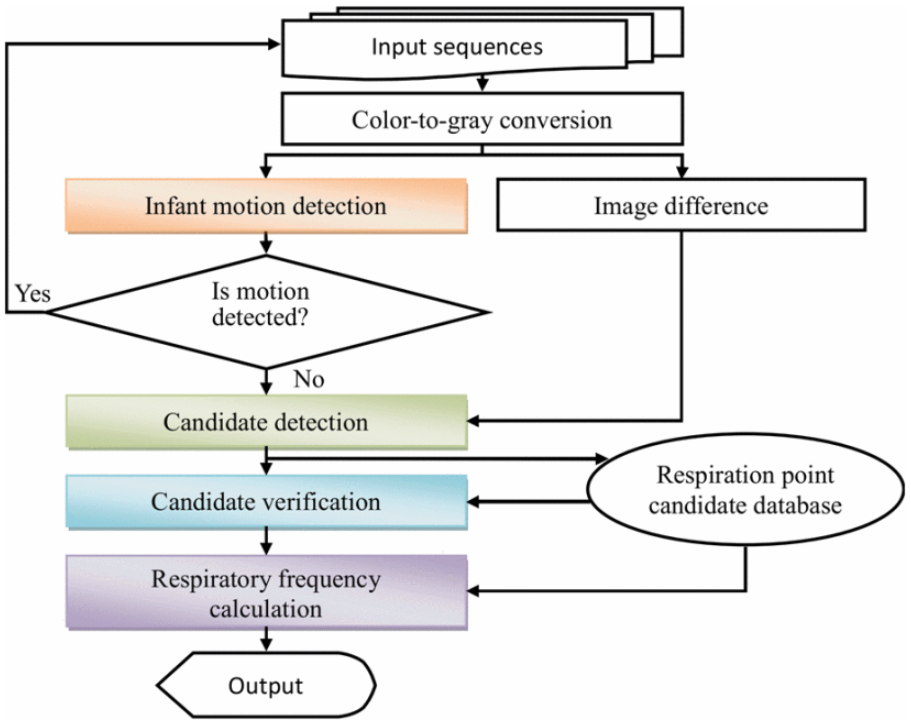
\includegraphics[width=0.45\linewidth]{fig-fang_vision-based_2015-01}}
    ~
    \subcaptionbox
        {嬰兒運動偵測
        \label{fig:fig-fang_vision-based_2015-02}}
        {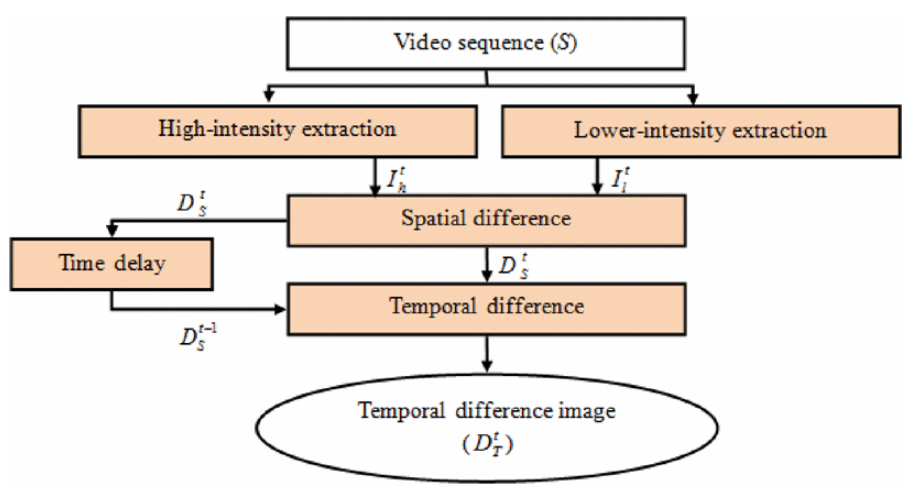
\includegraphics[width=0.45\linewidth]{fig-fang_vision-based_2015-02}}
    \caption{Fang系統流程圖~\cite{fang_vision-based_2015}}
    \label{fig:fig-fang_vision-based_2015}
\end{figure}

Liu等人~\cite{liu_video-based_2017}
利用夜視攝影機拍攝在嬰兒床內的嬰兒,
判斷其呼吸頻率異常與否。
此系統主要包含三個部分:
(1)影片收集:
為\cref{fig:fig-liu_video-based_2017-01}中的前兩項,
透過夜視攝影機連接到Artik板以收集嬰兒影片;
(2)呼吸偵測演算法:
為\cref{fig:fig-liu_video-based_2017-01}中的第三及四項,
包含了使用Eulerian Magnification技術放大影片中的細微運動,
以監測拍攝對象之胸部運動,
而若經正規化之像素差異值低於設定閥值,
則判斷為呼吸頻率異常;
(3)警示:
為\cref{fig:fig-liu_video-based_2017-01}中的最後兩項,
透過Twilio在演算法偵測到緊急狀況時,
向父母手機發出警報。
\fig[0.7][fig:fig-liu_video-based_2017-01][!hbt]{fig-liu_video-based_2017-01.png}[Liu系統設計圖~\cite{liu_video-based_2017}][Liu系統設計圖~\cite{liu_video-based_2017}]

Gallo等人~\cite{gallo_marrsids_2019}提出名為MARRSIDS的模型(架構如\cref{fig:fig-gallo_marrsids_2019}),
其利用OpenCV之Haar-Like Features偵測嬰兒面部特徵,
若未偵測到其臉部,
則認為嬰兒可能位於不良姿勢,
需發出警示;
而若偵測到嬰兒臉部且為睜眼狀態,
則代表其處於清醒狀態,
並非處於風險中。
\fig[0.9][fig:fig-gallo_marrsids_2019][!hbt]{fig-gallo_marrsids_2019.png}[MARRSIDS模型架構圖~\cite{gallo_marrsids_2019}][MARRSIDS模型架構圖~\cite{gallo_marrsids_2019}]

Wang等人~\cite{wang_multi-task_2019}
提出用以偵測嬰兒臉部遮擋的貝氏深度神經網路架構(\cref{fig:fig-wang_multi-task_2019-01}),
共包含四項子任務:
(1)眼睛、鼻子或嘴巴是否可見,
(2)不可見的原因是否為被外物(如:枕頭)遮擋,
(3)眼睛睜開與否,
及(4)五個臉部座標之位置。
此框架使用了損失函數進行訓練,
並考慮不同偵測任務間的不確定性,
且有別於現有不專注於嬰兒影像的研究,
此方法使用MobileNetV2針對自行收集之YunInfants資料集進行嬰兒頭部影像分析。
\fig[0.7][fig:fig-wang_multi-task_2019-01][!hbt]{fig-wang_multi-task_2019-01.png}[Wang系統之網路架構~\cite{wang_multi-task_2019}][Wang系統之網路架構~\cite{wang_multi-task_2019}]

Bharati等人~\cite{bharati_efficient_2021}
開發基於卷積神經網絡之嬰兒睡眠姿勢電腦視覺系統,
以評估仰臥(正常狀態)、從仰臥轉換到趴臥(警示狀態)及趴臥(危險狀態)三種姿勢
(如\cref{fig:fig-bharati_efficient_2021-01}),
並於嬰兒呈現趴臥時,
透過手機提醒照護人員。
此系統完整架構見\cref{fig:fig-bharati_efficient_2021-02},
其中卷積神經網路部分之架構如\cref{fig:fig-bharati_efficient_2021-03}:
首先,輸入經轉換的2D嬰兒灰階影像;
接著,經過多次的卷積層及最大池化層;
再傳入全連接層後,
最終輸出嬰兒的三種睡眠姿勢機率值。
由於目前未有公開之嬰兒姿勢資料集,
故此研究所使用的影像資料為和真實嬰兒相同比例之娃娃。
\fig[0.7][fig:fig-bharati_efficient_2021-01][!hbt]{fig-bharati_efficient_2021-01.png}[Bharati系統之嬰兒睡眠姿勢分類~\cite{bharati_efficient_2021}][Bharati系統之嬰兒睡眠姿勢分類~\cite{bharati_efficient_2021}]
\begin{figure}[!hbt]
    \centering
    \subcaptionbox
        {完整系統
        \label{fig:fig-bharati_efficient_2021-02}}
        {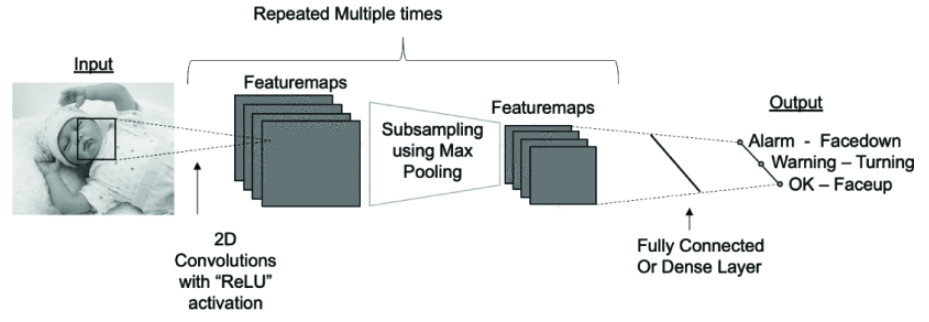
\includegraphics[width=0.9\linewidth]{fig-bharati_efficient_2021-02}}
    ~
    \subcaptionbox
        {卷積神經網路
        \label{fig:fig-bharati_efficient_2021-03}}
        {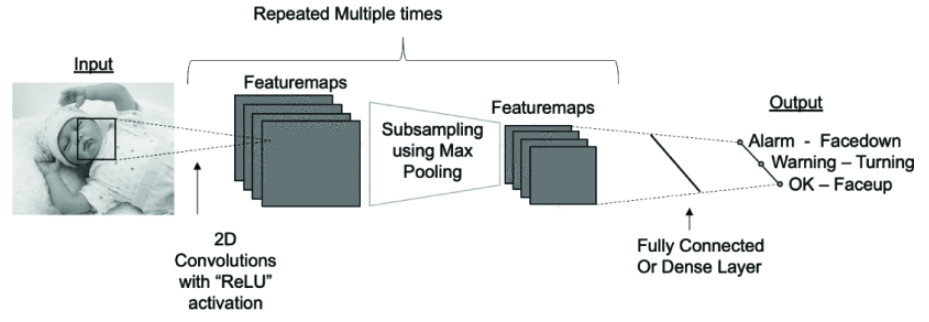
\includegraphics[width=0.9\linewidth]{fig-bharati_efficient_2021-03}}
    \caption{Bharati系統架構圖~\cite{bharati_efficient_2021}}
    \label{fig:fig-bharati_efficient_2021}
\end{figure}

現有研究中,
視覺化之嬰兒監測系統多關注其呼吸運動、面部特徵或單一姿勢,
而未有辨識嬰兒常見動作之研究,
故我們提出一可偵測嬰兒基礎姿勢及面部遮擋之危險監測系統。

\section{殘差神經網路}
既有研究中~\cite{simonyan_very_2015, szegedy_going_2015, ioffe_batch_2015},
可知卷積神經網路其深度至關重要,
在ImageNet資料集中結果表現良好的網路皆為十六至三十層之深層網路。

然而,
當訓練更深層的神經網路時,
卻會出現退化問題,
亦即隨著網路深度的增加,
準確率達飽和後,
反而迅速下降,
而這樣的結果並非因過度擬合所致,
如\cref{fig:fig-residual-learning-0}可看到兩個不同層數的網路其訓練及測試誤差值。
\fig[0.9][fig:fig-residual-learning-0][!hbt]{fig-residual-learning-0.png}[網路深度與訓練誤差關係~\cite{he_deep_2016}][網路深度與訓練誤差關係~\cite{he_deep_2016}]

因此,He等人~\cite{he_deep_2016}
提出使用深度殘差學習(\cref{fig:fig-residual-learning-1})的網路架構,
利用shortcut connection執行identity mapping,
且不需要增加額外的參數,
亦即不增加計算複雜度。
\fig[0.7][fig:fig-residual-learning-1][!hbt]{fig-residual-learning-1.png}[殘差學習~\cite{he_deep_2016}][殘差學習~\cite{he_deep_2016}]

此研究中,
通過訓練ImageNet評估不同層數之普通網路與殘差網路,
由\cref{fig:fig-residual-learning-2}(左)可觀察到普通網路中34層卻比18層有更高的驗證誤差,
而\cref{fig:fig-residual-learning-2}(右)則可看出殘差網路中34層相對於18層有較低的訓練誤差,
此結果說明退化問題獲得了解決。
而文中亦透過訓練CIFAK-10進行更多的比較,
\cref{fig:fig-residual-learning-3}(左)為普通網路不同層數之誤差曲線圖,
\cref{fig:fig-residual-learning-3}(中)為殘差網路不同層數其誤差曲線圖,
\cref{fig:fig-residual-learning-3}(右)則為使用110層及1202層殘差網路之誤差曲線圖。
\fig[0.9][fig:fig-residual-learning-2][!hbt]{fig-residual-learning-2.png}[在ImageNet上訓練之誤差曲線圖~\cite{he_deep_2016}][在ImageNet上訓練之誤差曲線圖~\cite{he_deep_2016}]
\fig[0.9][fig:fig-residual-learning-3][!hbt]{fig-residual-learning-3.png}[在CIFAK-10上訓練之誤差曲線圖~\cite{he_deep_2016}][在CIFAK-10上訓練之誤差曲線圖~\cite{he_deep_2016}]

最終,
本研究以152層之殘差網路在ILSVRC 2015中獲得第一名,
此網路比VGG網路深八倍,
卻仍擁有較低的複雜度。

\section{人臉偵測演算法}
本節將探討近年著名之兩項人臉偵測演算法:
MTCNN及RetinaFace,
以應用在本研究中嬰兒臉部偵測部分。

\subsection{MTCNN}
MTCNN~\cite{zhang_joint_2016}是由Zhang等人於2016年提出的一種多任務級聯卷積神經網路,
可以同時處理人臉偵測及對齊任務,
並提出online hard sample mining策略以提升效能。

此演算法為包含三階段級聯架構的深度卷積網路,
架構如\cref{fig:fig-mtcnn-framework}:
第一階段為全卷積網路構成之proposal network(P-Net),
用來獲得人臉區域的候選窗口及其邊界框回歸向量,
根據此估計回歸向量校準候選者,
再以非極大值抑制合併高度重疊的候選者;
而第二階段,
所有候選者皆饋送至另一個稱為refine network(R-Net)的卷積神經網路,
以進一步拒絕大量錯誤候選者,
並使用邊界框回歸進行校準及非極大值抑制;
第三階段中,
則利用output network(O-Net)輸出五個臉部的座標位置,
其類似於第二階段,
但目標為識別受更多監督的人臉區域。
由\cref{fig:fig-mtcnn-pipeline},
可清楚看出此網路是以粗到細的方式預測人臉及座標位置。
\fig[0.9][fig:fig-mtcnn-framework][!hbt]{fig-mtcnn-framework.PNG}[MTCNN架構圖~\cite{zhang_joint_2016}][MTCNN架構圖~\cite{zhang_joint_2016}]
\fig[0.6][fig:fig-mtcnn-pipeline][!hbt]{fig-mtcnn-pipeline.PNG}[MTCNN pipline~\cite{zhang_joint_2016}][MTCNN pipline~\cite{zhang_joint_2016}]

為了評估人臉偵測效果,
此網路與FDDB及WIDER FACE中的其他方法進行比較,
結果如\cref{fig:fig-mtcnn-result-1},
可看出此演算法確實優於其他方法。
而為了評估人臉對齊效果,
此網路亦與多種方法進行比較,
結果如\cref{fig:fig-mtcnn-result-2},
可看出此演算法雖在嘴角定位較不具優勢,
但其他部分仍優於多數方法。
\fig[0.7][fig:fig-mtcnn-result-1][!hbt]{fig-mtcnn-result-1.PNG}[MTCNN偵測人臉之效果比較~\cite{zhang_joint_2016}][MTCNN偵測人臉之效果比較~\cite{zhang_joint_2016}]
\fig[0.9][fig:fig-mtcnn-result-2][!hbt]{fig-mtcnn-result-2.PNG}[MTCNN人臉對齊之效果比較~\cite{zhang_joint_2016}][MTCNN人臉對齊之效果比較~\cite{zhang_joint_2016}]

\subsection{RetinaFace}
由Deng等人於2020年提出的RetinaFace~\cite{deng_retinaface_2020},
為一種single-shot、multi-level人臉定位方法,
其基於影像平面之點回歸整合了人臉框預測、2D人臉標示定位及3D頂點回歸。

此模型架構(見\cref{fig:fig-retinaface-framework})中,主要由三個部分組成:
(1)feature pyramid network、(2)context head module及(3)cascade multi-task loss。
首先,由feature pyramid network輸入影像,並輸出五個不同比例的特徵圖;
接著,context head module獲得這些特徵圖以計算多任務的損失。
亦即第一個模組會從一般的anchor預測範圍框,
而後第二個模組利用第一個模組迴歸出的anchor以預測更精準的範圍框。
\fig[0.9][fig:fig-retinaface-framework][!hbt]{fig-retinaface-framework.PNG}[RetinaFace架構圖~\cite{deng_retinaface_2020}][RetinaFace架構圖~\cite{deng_retinaface_2020}]

本篇論文展示了RetinaFace和其他29種人臉偵測演算法平均準確度之比較,
如\cref{fig:fig-retinaface-ap}所示,
此演算法擁有91.7\%的良好結果。
\fig[0.7][fig:fig-retinaface-ap][!hbt]{fig-retinaface-ap.PNG}[RetinaFace偵測人臉之效果比較~\cite{deng_retinaface_2020}][RetinaFace偵測人臉之效果比較~\cite{deng_retinaface_2020}]

\end{document}